%\section{Computational Methods and Software}
\label{sec:software}

The previous chapter described a series of models 
for the system of interest. 
%These models are too 
%complicated to solve exactly, and must instead be 
%instantiated with software to produce a numerical 
%result. 
This chapter details the numerical formulation
and simulation of these models. It begins with a 
discussion of the numerical discretization of the equations 
of interest. The mesh discretization is then described. 
Next, the scientific software in which these numerical 
models are used is discussed. Finally, the tool
chain and supercomputer systems are briefly introduced. 

\section{Discretization Scheme}

A finite element method (FEM) is used to numerically solve the
Navier-Stokes equations on a computer. 
Typically, this requires that the equations
in section~\ref{sub_sec:ns_en} be cast into a weak form. Manipulating
these partial differential equations into a variational formulation is
accomplished by multiplying the equations by appropriate test functions
and integrating over the domain, $\Omega$. The resulting weak problem is
to find, $(u,p,T) \in H^1(\Omega)^3 \times L_2(\Omega) \times
H^1(\Omega)$ such that 

%
% http://www.numerik.uni-hd.de/Oberwolfach-Seminar/CFD-Course.pdf
%
\begin{align}
  (\frac{\partial u}{\partial t}, v) + (u \cdot \nabla u,v) + \nu
   (\nabla u, \nabla v)  
  -(p,\nabla \cdot u) &= (gT'/T_0,v)
 \label{eqn:ns_weak} \\
 (\nabla \cdot u,q) &= 0
 \label{eqn:cont_weak} \\
 (\frac{\partial T}{\partial t}, w) + (u \cdot \nabla T, w) + (k \, \nabla
 T, \nabla w) &= 0.\label{eqn:en_weak}
\end{align}

$\forall (v,q,w) \in H^1(\Omega)^3 \times L_2(\Omega) \times
H^1(\Omega)$, where $(u,v) = \int_\Omega u \cdot v \, dx$.  
Some of the simulations presented here were conducted under
steady conditions, for which the $\frac{\partial}{\partial t}$ terms
vanish. An FEM scheme is obtained by posing the weak form in
terms of discrete subspaces of the function spaces specified above
defined using piecewise-polynomial basis functions. All of the
simulations discussed in this work were accomplished using 
linear basis functions for both the velocity and pressure. 
Typically, the use of equal order elements for velocity and pressure is
ruled out in the standard Galerkin FEM formulation by the Babuska-Brezzi
condition\cite{bb-cond}. 
However, the weak form equations shown above are stable with equal-order
elements for velocity and pressure due to the introduction of streamline
upwind/Petrov-Galerkin (SUPG) stabilization terms as first described by
Hughes\cite{Hughes198685,supg} and extended to natural convection as in
Becker and Braack\cite{Becker2002428}. These stabilization terms add
artificial dissipation that approaches zero as the residual
converges. This scheme is ``consistent'' because the underlying order of
convergence of the numerical method is not affected\cite{hughes2000finite}. 

This stabilization is accomplished by introducing an additional term,
$\langle Lc,S\phi \rangle_\tau$, to the weak form defined in Equations
\ref{eqn:ns_weak}-\ref{eqn:en_weak}. Here $L()$ is the operator for the PDEs
in \ref{sub_sec:ns_en}, and S() is a stabilization operator
which is chosen to be the negative adjoint of the differential terms of
$L()$, and $c$ and $\phi$ are state and test functions, i.e. 
$ c= (u,p,T)$, and $\phi = ( v,w,q )$. 
The angle brackets $\langle \cdot,\cdot \rangle$ signify integration of
the element interiors for each of the K elements, that is:
\begin{equation}
 \langle u,v \rangle_\tau = \sum_K \tau_K(u,v)_K.
\end{equation}
This results in three stabilization parameters, $\tau_P, \tau_v, \tau_T$ 
which are selected as proposed by Becker and Braack. 
A full derivation of the weak form and stabilization terms are provided
in Appendix \ref{app:stab}. 

The system of ODEs are discretized in time using the 
backward Euler method\cite{moin2010fundamentals}. The time interval
$(0,T)$ is sliced into $N_t$ steps of 
uniform temporal length,  $\Delta t$, where $n = 0,\dots,N_t$. 
This has the form, 
\begin{equation}
 y_{n+1} = y_n + \Delta t \, f(y_{n+1},t_{n+1}).
\end{equation}
As $f$ is non-linear, a Newton-Raphson method is used to solve the
resulting implicit nonlinear problem. While an iterative method is
significantly more computationally expensive per timestep than a similar
explicit method, the method was selected due to its unconditional
stability and ease of statistical sampling for a uniform timestep. 


%
% gave not completely described numerical methods
% for instance, have not indicated the stabilization schemes
% do not need complete equations, but should permit someone to access 
% the literature and construct precisely the numerical formulations used
%


\section{Mesh Discretization}

%
% what about mesh...
%
The domain's described in section~\ref{sec:bc} are
consistently discretized. The domain extents
are scaled by system diameter but the same number of grid points are used
for every simulation. Thus, while the ratio of the domain length to system
diameter remains fixed, the grid spacing increases proportionally with
domain length. 

The mesh has a uniform spacing in the lateral directions, except for a
single refinement in the region of the vanes. Typically, the grid is 
roughly one hundred points in the streamwise and spanwise directions
before the refinement. The refinement halves the spacing (doubles the
number of points) in all three
coordinate directions, \{x,y,z\} in this region. The refinement is made
from the ground to 1.5 times the height of the vanes and cone. 

The mesh is non-uniform in height to
resolve the boundary layer. This is accomplished by redistributing a
mesh uniform in height, z, according to,
\begin{equation}
 z = \begin{cases} C_1(z-L_z)+L_z,& \text{if } z \geq z_\delta\\
      C_2 \text{ exp}(C_3 z - 1),                 & \text{otherwise}
     \end{cases}
\end{equation}

where $z_\delta$ is the chosen height of the boundary layer mesh, and
$C_1-C_3$ are scaling coefficients\todo{show coefficients}. 
This gives the mesh an exponentially
varying character, with the coefficients chosen to ensure ten or more
points in the boundary layer, isotropic spacing in cells outside of
it, and smooth blending between these two regimes. Each boundary layer
spacing was tested against a finer spacing to ensure that the results
were not sensitive to the choice of spacing. A horizontal slice though a
representative domain is shown in Figure \ref{fig:meshing}. The single
refinement in the region of the vanes is visible, along with the finer
meshed boundary layer region near the ground. 

  \begin{figure}[!htb]
    \begin{center}
     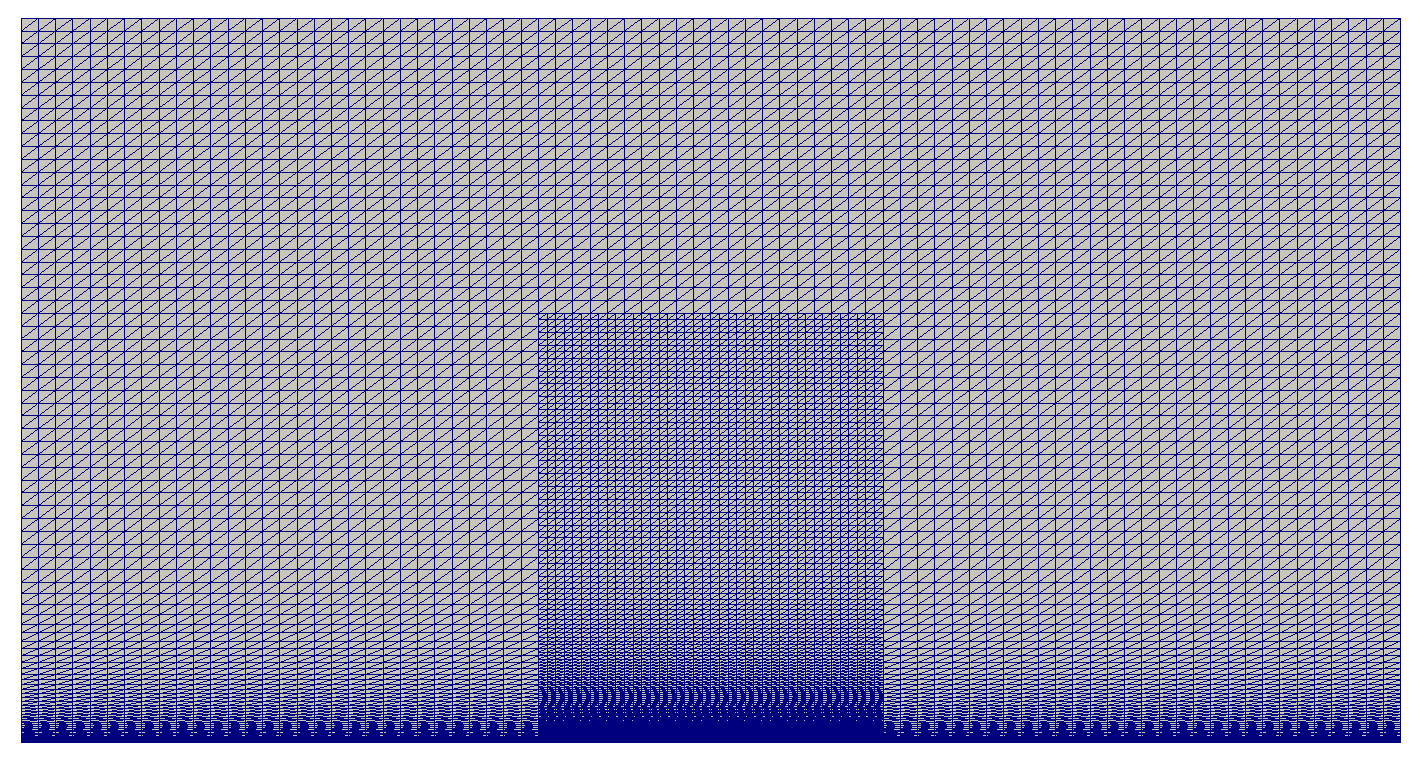
\includegraphics[width = 10 cm]{figs/meshing}
     \caption{Horizontal slide through the domain, to show a
     representative meshing. The single refinement region around the
     vanes is visible, along with the finer boundary layer mesh near the
     ground.}
     \label{fig:meshing}
    \end{center}
  \end{figure}

Finally, the diffusivities are proportionally
scaled with grid size to ensure that the cell Reynolds number, 
\begin{equation}
 \text{Re}_\text{cell} = \frac{\text{max}(\Delta x,\Delta y) u}{\nu_T}
\end{equation}
 is maintained for every simulation, to ensure stability.


%% hmin = 0.001  
%% hmax = 0.4  
%% zb = 2.0
%% hrat = ${/ ${mesh-options/hmax} ${mesh-options/hmin}}
%% zmax = ${mesh-options/domain_x3_max}
%% loghrat = ${= log ${mesh-options/hrat}}
%% c2 = ${/ ${mesh-options/zb} ${- ${mesh-options/hrat} 1}} 
%% zetab = ${/ ${mesh-options/zmax} ${+ 1 ${/ ${- ${mesh-options/zmax} ${mesh-options/zb}} ${* ${mesh-options/c2} ${mesh-options/hrat} ${mesh-options/loghrat}}}}}
%% c3 = ${/ ${mesh-options/loghrat} ${mesh-options/zetab}}
%% mesh_nx3 = ${= ceil ${/ ${* ${mesh-options/zmax} ${mesh-options/c2} ${mesh-options/c3}} ${mesh-options/hmin}}}
%% c1 = ${* ${mesh-options/c2} ${mesh-options/c3} ${= exp ${* ${mesh-options/c3} ${mesh-options/zetab}}}}
%% redistribute = '{x}{y}{if(z>${mesh-options/zetab},${mesh-options/c1}*(z-${mesh-options/zmax})+${mesh-options/zmax},${mesh-options/c2}*(exp(${mesh-options/c3}*z)-1))}' 

%After operation, solutions are evaluated to ensure that 
%the qualitative character of the solution does not change.

\section{Software Stack}

The numerical approximations described above had been implemented using
the GRINS library\cite{GRINSpaper} by Bauman and Stogner using the
Libmesh\cite{libMeshPaper} FEM infrastructure. It was designed to
support multiphysics FEM applications, the reusability and extensibility
of mathematical modeling kernels, supporting interfaces to existing
solver and discretization libraries to enable modern solution
strategies, while, at the same time, retaining flexibility to
effectively address a wide range of science or engineering problems.  

GRINS provides a platform that enables powerful numerical algorithms
such as adjoint-based AMR, adaptive modeling, sensitivity analysis,
and, eventually, enabling uncertainty quantification. While few of these
capabilities are in use for the present work, they could be useful in
future investigations. 

GRINS stands for, ``General Reacting Incompressible Navier-Stokes'',
which roughly encapsulates the physical regimes it was originally
designed to simulate. GRINS is open-source, and available on
\hyperref[www.github.com/grinsfem/grins]{GitHub}. It is released 
under LGPL2.1.  GRINS is heavily unit tested, with over 60 tests
available to ensure the reliability of results regardless of install
platform. 

%The remainder of this section is devoted to
%discussing the underlying libraries used and the description of the
%GRINS framework.  
% PETSC\cite{petsc} trilinos\cite{trilinos}

% GRINS also uses the fparser\cite{fparser}
% library to support both parsing and compilation of mathematical
% functions into high 
% performance kernels. This capability allows for easy specification of
% boundary conditions, initial conditions, or constitutive equations from an input file. 

% Currently, libMesh has been scaled tens of thousands of cores and has
% been run on over 100,000 cores on the BG/Q machine Mira at Argonne National
% Lab\cite{libmesh-scaling}

%In principle, alternative software libraries/frameworks such as
%FEniCS\cite{fenics}, OpenFOAM\cite{openfoam}, etc. would likely be
%capable of simulating this regime. 


%
% INCLUDE IN THESIS
%
% \section{Solver Options}

% GRINS uses PETSC\cite{petsc} and trilinos\cite{trilinos} for numerical
% linear algebra, such as constructing and using sparse matrices, finding
% the iterative solution of linear systems, and for preconditioning.  

% While a variety of solver options have been tested in PETSC, all the
% results shown in this document use GMRES with block Jacobi for
% preconditioning\cite{Saad:2003} for the linear solve. 

% This uses the inverse of the diagonal block for that processor for
% preconditioning. 

% the preconditioner it's going to use to precondition the linear system
% for the solution of the diagonal block. To approximate this, incomplete
% LU factorization is used. 

% ILU(0) factorization



%% (11:41:54 AM) nick: ``-ksp_view -ksp_type gmres -pc_type bjacobi -sub_pc_type ilu -sub_pc_factor_levels 0''
%% (11:42:00 AM) Paul Bauman: OK
%% (11:42:17 AM) Paul Bauman: -pc_type is the preconditioner for the entire linear system
%% (11:42:25 AM) Paul Bauman: You're doing bjacobi = block Jacobi
%% (11:42:28 AM) nick: right
%% (11:42:36 AM) nick: and does anyone have a good reference I can learn this better? i feel as if I cant look this up, for some reason
%% (11:42:39 AM) Paul Bauman: That is just using the inverse of the diagonal block for that processor
%% (11:42:46 AM) Paul Bauman: Now
%% (11:42:55 AM) Paul Bauman: that is a linear solve
%% (11:43:17 AM) Paul Bauman: So you can use all the linear solver technology to solve or approximately that block
%% (11:43:24 AM) Paul Bauman: Hence, -sub_pc_type
%% (11:43:32 AM) hil left the room.
%% (11:43:46 AM) Paul Bauman: That's the preconditioner it's going to use to precondition the linear system for the solution of the diagonal block
%% (11:43:53 AM) Paul Bauman: You're telling it to use incomplete lu
%% (11:44:26 AM) Paul Bauman: Now the -sub_pc_factor_levels options applies to ilu
%% (11:44:28 AM) hil entered the room.
%% (11:44:44 AM) Paul Bauman: The incomplete part of imcomplete LU is about the level of fill you use
%% (11:45:05 AM) Paul Bauman: The more levels of fill you have, the more ``complete'' the incomplete LU will be
%% (11:45:08 AM) Paul Bauman: Does that make sense?
%% (11:45:23 AM) nick: no, that is where you lost me
%% (11:45:39 AM) nick: i dont think i know this level of fill
%% (11:46:17 AM) Paul Bauman: Check out Youssef Saad's book if more curious about the subject
%% (11:46:37 AM) nick: cool thanks
%% (11:46:38 AM) Paul Bauman: Suffice it to say, you heopfully shouldn't ever need to go past 3 or 4 levels of fill
%% (11:47:03 AM) Paul Bauman: Also, if you've got superlu installed with the PETSc, consider using -sub_pc_factor_mat_solver_package superlu
%% (11:47:15 AM) Paul Bauman: That's a *much* faster/better implementation than PETSc's


\section{Tool Chain and Simulation Custodianship}

Simulations are performed on the Texas Advanced Computing Center (TACC)
supercomputers Lonestar Four and Stampede. Run durations for transient
cases are typically twelve hours to perform several hundred timesteps. 
These runs are submitted to the production queue and are  
264-528 processing cores, 
or 22-44 nodes on Lonestar (with 12 cores per node), and a similar number
for Stampede. The runs typically have several million degrees of freedom (DoF), 
and the local number of DoF per core is maintained at $O(10^4)$. This was
selected due to memory constraints, after a strong scaling
analysis of the performance of the code on these resources, and
after consulting with the software developers.  \todo{add LS5}

After a run terminates, several scripts are automatically invoked. 
These scripts archive the run (outside of the volatile /scratch 
production directories) and simultaneously, label the concluded run with
unique metadata that defines the system environment, the jobs input
files and run definitions, and information detailing the
hypothesis or physics the job was intended to investigate. Finally, once
a week a script performs \textbf{rsync} on the entire archived database to
ensure more than single redundancy for the runs. 

In other words, the workflow is designed to permit rapid queuing of a
series of runs (in parallel) to investigate a variety of conditions or
scenario parameters. This capability is necessary for the optimization
campaign detailed in \ref{sec:results}, where running many concurrent
investigations are required to sample the configuration space.  

\section{Testing and Verification}

grid convergence?

regression tests in grins

validation (later)